\documentclass[english, 11pt]{article}\usepackage[]{graphicx}\usepackage[]{color}
%% maxwidth is the original width if it is less than linewidth
%% otherwise use linewidth (to make sure the graphics do not exceed the margin)
\makeatletter
\def\maxwidth{ %
  \ifdim\Gin@nat@width>\linewidth
    \linewidth
  \else
    \Gin@nat@width
  \fi
}
\makeatother

\definecolor{fgcolor}{rgb}{0.345, 0.345, 0.345}
\newcommand{\hlnum}[1]{\textcolor[rgb]{0.686,0.059,0.569}{#1}}%
\newcommand{\hlstr}[1]{\textcolor[rgb]{0.192,0.494,0.8}{#1}}%
\newcommand{\hlcom}[1]{\textcolor[rgb]{0.678,0.584,0.686}{\textit{#1}}}%
\newcommand{\hlopt}[1]{\textcolor[rgb]{0,0,0}{#1}}%
\newcommand{\hlstd}[1]{\textcolor[rgb]{0.345,0.345,0.345}{#1}}%
\newcommand{\hlkwa}[1]{\textcolor[rgb]{0.161,0.373,0.58}{\textbf{#1}}}%
\newcommand{\hlkwb}[1]{\textcolor[rgb]{0.69,0.353,0.396}{#1}}%
\newcommand{\hlkwc}[1]{\textcolor[rgb]{0.333,0.667,0.333}{#1}}%
\newcommand{\hlkwd}[1]{\textcolor[rgb]{0.737,0.353,0.396}{\textbf{#1}}}%
\let\hlipl\hlkwb

\usepackage{framed}
\makeatletter
\newenvironment{kframe}{%
 \def\at@end@of@kframe{}%
 \ifinner\ifhmode%
  \def\at@end@of@kframe{\end{minipage}}%
  \begin{minipage}{\columnwidth}%
 \fi\fi%
 \def\FrameCommand##1{\hskip\@totalleftmargin \hskip-\fboxsep
 \colorbox{shadecolor}{##1}\hskip-\fboxsep
     % There is no \\@totalrightmargin, so:
     \hskip-\linewidth \hskip-\@totalleftmargin \hskip\columnwidth}%
 \MakeFramed {\advance\hsize-\width
   \@totalleftmargin\z@ \linewidth\hsize
   \@setminipage}}%
 {\par\unskip\endMakeFramed%
 \at@end@of@kframe}
\makeatother

\definecolor{shadecolor}{rgb}{.97, .97, .97}
\definecolor{messagecolor}{rgb}{0, 0, 0}
\definecolor{warningcolor}{rgb}{1, 0, 1}
\definecolor{errorcolor}{rgb}{1, 0, 0}
\newenvironment{knitrout}{}{} % an empty environment to be redefined in TeX

\usepackage{alltt}
\usepackage[utf8]{inputenc}
\usepackage{booktabs}
\usepackage{booktabs}
\usepackage{longtable}
\usepackage{array}
\usepackage{multirow}
\usepackage[table]{xcolor}
\usepackage{wrapfig}
\usepackage{float}
\usepackage{colortbl}
\usepackage{pdflscape}
\usepackage{tabu}
\usepackage{threeparttable}
\usepackage[normalem]{ulem}
\IfFileExists{upquote.sty}{\usepackage{upquote}}{}
\begin{document}

\title{ARE 212 Midterm}
\author{Matthew Tadruno }

\maketitle

\newpage
\noindent \section*{Question 1} (Answers start below)



\begin{knitrout}\footnotesize
\definecolor{shadecolor}{rgb}{0.969, 0.969, 0.969}\color{fgcolor}\begin{kframe}
\begin{alltt}
\hlcom{# Setup ----}

\hlcom{# Packages }
\hlkwd{library}\hlstd{(pacman)}
\hlkwd{library}\hlstd{(knitr)}
\hlcom{# p_load examples}
\hlkwd{p_load}\hlstd{(dplyr, haven, readr, xtable, psych, magrittr)}
\hlkwd{p_load}\hlstd{(ggplot2, extrafont, Matrix)}

\hlcom{# Loading data }
\hlstd{directory}\hlkwb{<-}\hlstr{"/Users/matthewtarduno/Desktop/212/midterm/"}
\hlstd{raw} \hlkwb{<-}\hlkwd{read_csv}\hlstd{(}\hlkwd{paste0}\hlstd{(directory,} \hlstr{"data.csv"}\hlstd{),} \hlkwc{col_types}\hlstd{=}\hlkwd{cols}\hlstd{())}
\end{alltt}
\end{kframe}
\end{knitrout}


\begin{knitrout}\footnotesize
\definecolor{shadecolor}{rgb}{0.969, 0.969, 0.969}\color{fgcolor}\begin{kframe}
\begin{alltt}
\hlcom{# Cleaning Data ---- }

\hlcom{# note, I added a period dummy when I put the data into csv form. }

\hlcom{# Using the dummy.code() function of psych }
\hlstd{dummies}\hlkwb{<-}\hlkwd{as.data.frame}\hlstd{(}\hlkwd{dummy.code}\hlstd{(raw}\hlopt{$}\hlstd{state))}
\hlcom{# Clean dummy names }
\hlkwd{names}\hlstd{(dummies)}\hlkwb{<-}\hlkwd{gsub}\hlstd{(}\hlstr{' '}\hlstd{,} \hlstr{'\textbackslash{}\textbackslash{}.'}\hlstd{,} \hlkwd{names}\hlstd{(dummies))}


\hlcom{# Combine the two dataframes }
\hlstd{data}\hlkwb{<-}\hlkwd{as.data.frame}\hlstd{(}\hlkwd{c}\hlstd{(raw, dummies))}

\hlcom{#remove % sign }
\hlstd{data}\hlopt{$}\hlstd{emmigrant.ratio}\hlkwb{<-}\hlkwd{substr}\hlstd{(data}\hlopt{$}\hlstd{emmigrant.ratio,} \hlnum{1}\hlstd{,}
                             \hlkwd{nchar}\hlstd{(}\hlkwd{as.character}\hlstd{(data}\hlopt{$}\hlstd{emmigrant.ratio))}\hlopt{-}\hlnum{1}\hlstd{)}
\hlstd{data}\hlopt{$}\hlstd{emmigrant.ratio}\hlkwb{<-}\hlkwd{as.numeric}\hlstd{(data}\hlopt{$}\hlstd{emmigrant.ratio)}
\hlstd{data}\hlopt{$}\hlstd{emmigrant.ratio}\hlkwb{<-}\hlstd{data}\hlopt{$}\hlstd{emmigrant.ratio}\hlopt{/}\hlnum{100}
\end{alltt}
\end{kframe}
\end{knitrout}

\begin{knitrout}\footnotesize
\definecolor{shadecolor}{rgb}{0.969, 0.969, 0.969}\color{fgcolor}\begin{kframe}
\begin{alltt}
\hlcom{# Functions ----}

\hlstd{to_matrix} \hlkwb{<-} \hlkwa{function}\hlstd{(}\hlkwc{the_df}\hlstd{,} \hlkwc{vars}\hlstd{) \{}
  \hlstd{mat} \hlkwb{<-} \hlstd{the_df} \hlopt
    \hlkwd{select_}\hlstd{(}\hlkwc{.dots} \hlstd{= vars)} \hlopt
    \hlkwd{as.matrix}\hlstd{()}
  \hlkwd{return}\hlstd{(mat)}
\hlstd{\}}


\hlcom{# Function for OLS coefficient estimates}
\hlstd{b_ols} \hlkwb{<-} \hlkwa{function}\hlstd{(}\hlkwc{data}\hlstd{,} \hlkwc{y_var}\hlstd{,} \hlkwc{X_vars}\hlstd{,} \hlkwc{intercept} \hlstd{=} \hlnum{TRUE}\hlstd{) \{}
  \hlkwd{require}\hlstd{(dplyr)}

  \hlstd{y} \hlkwb{<-} \hlkwd{to_matrix}\hlstd{(}\hlkwc{the_df} \hlstd{= data,} \hlkwc{vars} \hlstd{= y_var)}
  \hlstd{X} \hlkwb{<-} \hlkwd{to_matrix}\hlstd{(}\hlkwc{the_df} \hlstd{= data,} \hlkwc{vars} \hlstd{= X_vars)}

  \hlcom{# Use intercept arument }
  \hlkwa{if} \hlstd{(intercept} \hlopt{==} \hlstd{T) \{}
    \hlstd{X} \hlkwb{<-} \hlkwd{cbind}\hlstd{(}\hlnum{1}\hlstd{, X)}
    \hlkwd{colnames}\hlstd{(X)} \hlkwb{<-} \hlkwd{c}\hlstd{(}\hlstr{"intercept"}\hlstd{, X_vars)}
  \hlstd{\}}

  \hlcom{# Calculate, return beta hat}
  \hlstd{beta_hat} \hlkwb{<-} \hlkwd{solve}\hlstd{(}\hlkwd{t}\hlstd{(X)} \hlopt \hlstd{X)} \hlopt \hlkwd{t}\hlstd{(X)} \hlopt \hlstd{y}
  \hlkwd{return}\hlstd{(beta_hat)}
\hlstd{\}}


\hlcom{# This function returns additional info about regression in df }
\hlstd{ols} \hlkwb{<-} \hlkwa{function}\hlstd{(}\hlkwc{data}\hlstd{,} \hlkwc{y_var}\hlstd{,} \hlkwc{X_vars}\hlstd{,} \hlkwc{intercept} \hlstd{= T) \{}

  \hlcom{# Turn data into matrices}
  \hlstd{y} \hlkwb{<-} \hlkwd{to_matrix}\hlstd{(data, y_var)}
  \hlstd{X} \hlkwb{<-} \hlkwd{to_matrix}\hlstd{(data, X_vars)}

  \hlcom{# Add intercept based on arg}
  \hlkwa{if} \hlstd{(intercept} \hlopt{==} \hlstd{T) X} \hlkwb{<-} \hlkwd{cbind}\hlstd{(}\hlnum{1}\hlstd{, X)}


  \hlstd{n} \hlkwb{<-} \hlkwd{nrow}\hlstd{(X)}
  \hlstd{k} \hlkwb{<-} \hlkwd{ncol}\hlstd{(X)}

  \hlcom{# Estimate coefficients usinf above function }
  \hlstd{b} \hlkwb{<-} \hlkwd{b_ols}\hlstd{(data, y_var, X_vars, intercept)}

  \hlcom{# Calculate OLS residuals}
  \hlstd{e} \hlkwb{<-} \hlstd{y} \hlopt{-} \hlstd{X} \hlopt \hlstd{b}

  \hlcom{# Calculate sample var }
  \hlstd{s2} \hlkwb{<-} \hlstd{(}\hlkwd{t}\hlstd{(e)} \hlopt \hlstd{e)} \hlopt{/} \hlstd{(n}\hlopt{-}\hlstd{k)}

  \hlstd{XX_inv} \hlkwb{<-} \hlkwd{solve}\hlstd{(}\hlkwd{t}\hlstd{(X)} \hlopt \hlstd{X)}

  \hlstd{se} \hlkwb{<-} \hlkwd{sqrt}\hlstd{(s2} \hlopt{*} \hlkwd{diag}\hlstd{(XX_inv))}

  \hlcom{# Vector of _t_ statistics}
  \hlstd{t_stats} \hlkwb{<-} \hlstd{(b} \hlopt{-} \hlnum{0}\hlstd{)} \hlopt{/} \hlstd{se}
  \hlcom{# Calculate the p-values}
  \hlstd{p_values} \hlkwb{=} \hlkwd{pt}\hlstd{(}\hlkwc{q} \hlstd{=} \hlkwd{abs}\hlstd{(t_stats),} \hlkwc{df} \hlstd{= n}\hlopt{-}\hlstd{k,} \hlkwc{lower.tail} \hlstd{= F)} \hlopt{*} \hlnum{2}
  \hlcom{# table of results}
  \hlstd{results} \hlkwb{<-} \hlkwd{data.frame}\hlstd{(}
    \hlkwc{effect} \hlstd{=} \hlkwd{rownames}\hlstd{(b),}
    \hlkwc{coef} \hlstd{=} \hlkwd{as.vector}\hlstd{(b)} \hlopt \hlkwd{round}\hlstd{(}\hlnum{3}\hlstd{),}
    \hlkwc{std_error} \hlstd{=} \hlkwd{as.vector}\hlstd{(se)} \hlopt \hlkwd{round}\hlstd{(}\hlnum{3}\hlstd{),}
    \hlkwc{t_stat} \hlstd{=} \hlkwd{as.vector}\hlstd{(t_stats)} \hlopt \hlkwd{round}\hlstd{(}\hlnum{3}\hlstd{),}
    \hlkwc{p_value} \hlstd{=} \hlkwd{as.vector}\hlstd{(p_values)} \hlopt \hlkwd{round}\hlstd{(}\hlnum{4}\hlstd{)}
  \hlstd{)}
  \hlkwd{return}\hlstd{(results)}
\hlstd{\}}
\end{alltt}
\end{kframe}
\end{knitrout}


\begin{knitrout}\footnotesize
\definecolor{shadecolor}{rgb}{0.969, 0.969, 0.969}\color{fgcolor}\begin{kframe}
\begin{alltt}
\hlcom{# R2 Functions ---- }

\hlstd{demean} \hlkwb{<-} \hlkwa{function}\hlstd{(}\hlkwc{N}\hlstd{) \{}
  \hlstd{i} \hlkwb{<-} \hlkwd{matrix}\hlstd{(}\hlkwc{data} \hlstd{=} \hlnum{1}\hlstd{,} \hlkwc{nrow} \hlstd{= N)}
  \hlstd{A} \hlkwb{<-} \hlkwd{diag}\hlstd{(N)} \hlopt{-} \hlstd{(}\hlnum{1}\hlopt{/}\hlstd{N)} \hlopt{*} \hlstd{i} \hlopt \hlkwd{t}\hlstd{(i)}
  \hlkwd{return}\hlstd{(A)}
\hlstd{\}}


\hlstd{residuals} \hlkwb{<-} \hlkwa{function}\hlstd{(}\hlkwc{data}\hlstd{,} \hlkwc{y_var}\hlstd{,} \hlkwc{X_vars}\hlstd{,} \hlkwc{intercept} \hlstd{=} \hlnum{TRUE}\hlstd{) \{}
  \hlkwd{require}\hlstd{(dplyr)}
  \hlstd{y} \hlkwb{<-} \hlkwd{to_matrix}\hlstd{(}\hlkwc{the_df} \hlstd{= data,} \hlkwc{vars} \hlstd{= y_var)}
  \hlstd{X} \hlkwb{<-} \hlkwd{to_matrix}\hlstd{(}\hlkwc{the_df} \hlstd{= data,} \hlkwc{vars} \hlstd{= X_vars)}
  \hlkwa{if} \hlstd{(intercept} \hlopt{==} \hlstd{T) \{}
    \hlstd{X} \hlkwb{<-} \hlkwd{cbind}\hlstd{(}\hlnum{1}\hlstd{, X)}
    \hlkwd{colnames}\hlstd{(X)} \hlkwb{<-} \hlkwd{c}\hlstd{(}\hlstr{"intercept"}\hlstd{, X_vars)}
  \hlstd{\}}
  \hlstd{n} \hlkwb{<-} \hlkwd{nrow}\hlstd{(X)}
  \hlstd{resids} \hlkwb{<-} \hlstd{(}\hlkwd{diag}\hlstd{(n)} \hlopt{-} \hlstd{X} \hlopt \hlkwd{solve}\hlstd{(}\hlkwd{t}\hlstd{(X)} \hlopt \hlstd{X)} \hlopt \hlkwd{t}\hlstd{(X))} \hlopt \hlstd{y}
  \hlkwd{return}\hlstd{(resids)}
\hlstd{\}}


\hlstd{r2_ols} \hlkwb{<-} \hlkwa{function}\hlstd{(}\hlkwc{data}\hlstd{,} \hlkwc{y_var}\hlstd{,} \hlkwc{X_vars}\hlstd{) \{}

  \hlstd{y} \hlkwb{<-} \hlkwd{to_matrix}\hlstd{(data,} \hlkwc{vars} \hlstd{= y_var)}
  \hlstd{X} \hlkwb{<-} \hlkwd{to_matrix}\hlstd{(data,} \hlkwc{vars} \hlstd{= X_vars)}
  \hlcom{# Add intercept column to X}
  \hlstd{X} \hlkwb{<-} \hlkwd{cbind}\hlstd{(}\hlnum{1}\hlstd{, X)}

  \hlstd{N} \hlkwb{<-} \hlkwd{nrow}\hlstd{(X)}
  \hlstd{K} \hlkwb{<-} \hlkwd{ncol}\hlstd{(X)}

  \hlcom{# Calculate the residuals}
  \hlstd{e} \hlkwb{<-} \hlkwd{residuals}\hlstd{(data, y_var, X_vars)}
  \hlcom{# Calculate the y_star (demeaned y)}
  \hlstd{y_star} \hlkwb{<-} \hlkwd{demean}\hlstd{(N)} \hlopt \hlstd{y}

  \hlcom{# Calculate r-squared values}
  \hlstd{r2_uc}  \hlkwb{<-} \hlnum{1} \hlopt{-} \hlkwd{t}\hlstd{(e)} \hlopt \hlstd{e} \hlopt{/} \hlstd{(}\hlkwd{t}\hlstd{(y)} \hlopt \hlstd{y)}
  \hlstd{r2}     \hlkwb{<-} \hlnum{1} \hlopt{-} \hlkwd{t}\hlstd{(e)} \hlopt \hlstd{e} \hlopt{/} \hlstd{(}\hlkwd{t}\hlstd{(y_star)} \hlopt \hlstd{y_star)}
  \hlstd{r2_adj} \hlkwb{<-} \hlnum{1} \hlopt{-} \hlstd{(N}\hlopt{-}\hlnum{1}\hlstd{)} \hlopt{/} \hlstd{(N}\hlopt{-}\hlstd{K)} \hlopt{*} \hlstd{(}\hlnum{1} \hlopt{-} \hlstd{r2)}

  \hlkwd{return}\hlstd{(}\hlkwd{c}\hlstd{(}\hlstr{"r2_uc"} \hlstd{= r2_uc,} \hlstr{"r2"} \hlstd{= r2,} \hlstr{"r2_adj"} \hlstd{= r2_adj))}
\hlstd{\}}
\end{alltt}
\end{kframe}
\end{knitrout}


\newpage
\noindent \section*{Question 1 Part 1} Estimate model (1) via OLS. \\
\vspace{2mm}
\newline
\noindent These results do not match those from column 1 of the paper. 
The coefficient on log corn yield is \textbf{0.008} and the adjusted R-Squared value is \textbf{0.3212}.
The coefficient on log corn plus wheat yield is \textbf{0.008} and the adjusted R-Squared value is \textbf{0.3215}. 

\begin{knitrout}\footnotesize
\definecolor{shadecolor}{rgb}{0.969, 0.969, 0.969}\color{fgcolor}\begin{kframe}
\begin{alltt}
\hlcom{# Question 1 ----}

\hlkwd{ols}\hlstd{(}\hlkwc{data} \hlstd{= data,} \hlkwc{y} \hlstd{=} \hlstr{"emmigrant.ratio"}\hlstd{,} \hlkwc{X} \hlstd{=} \hlkwd{c}\hlstd{(}\hlstr{"log.corn"}\hlstd{,} \hlstr{"period"}\hlstd{))}
\end{alltt}


{\ttfamily\noindent\color{warningcolor}{\#\# Warning in s2 * diag(XX\_inv): Recycling array of length 1 in array-vector arithmetic is deprecated.\\\#\#\ \  Use c() or as.vector() instead.}}\begin{verbatim}
##      effect   coef std_error t_stat p_value
## 1 intercept  0.063     0.005 11.864  0.0000
## 2  log.corn  0.008     0.005  1.571  0.1214
## 3    period -0.037     0.007 -5.545  0.0000
\end{verbatim}
\begin{alltt}
\hlkwd{r2_ols}\hlstd{(}\hlkwc{data} \hlstd{= data,} \hlkwc{y} \hlstd{=} \hlstr{"emmigrant.ratio"}\hlstd{,} \hlkwc{X} \hlstd{=} \hlkwd{c}\hlstd{(}\hlstr{"log.corn"}\hlstd{,} \hlstr{"period"}\hlstd{))}
\end{alltt}
\begin{verbatim}
##     r2_uc        r2    r2_adj 
## 0.8067434 0.3427066 0.3211560
\end{verbatim}
\begin{alltt}
\hlcom{#lm(data$emmigrant.ratio ~ data$log.corn + data$period)}

\hlkwd{ols}\hlstd{(}\hlkwc{data} \hlstd{= data,} \hlkwc{y} \hlstd{=} \hlstr{"emmigrant.ratio"}\hlstd{,} \hlkwc{X} \hlstd{=} \hlkwd{c}\hlstd{(}\hlstr{"log.corn.wheat"}\hlstd{,} \hlstr{"period"}\hlstd{))}
\end{alltt}


{\ttfamily\noindent\color{warningcolor}{\#\# Warning in s2 * diag(XX\_inv): Recycling array of length 1 in array-vector arithmetic is deprecated.\\\#\#\ \  Use c() or as.vector() instead.}}\begin{verbatim}
##           effect   coef std_error t_stat p_value
## 1      intercept  0.063     0.005 11.523  0.0000
## 2 log.corn.wheat  0.008     0.005  1.580  0.1192
## 3         period -0.037     0.007 -5.529  0.0000
\end{verbatim}
\begin{alltt}
\hlkwd{r2_ols}\hlstd{(}\hlkwc{data} \hlstd{= data,} \hlkwc{y} \hlstd{=} \hlstr{"emmigrant.ratio"}\hlstd{,} \hlkwc{X} \hlstd{=} \hlkwd{c}\hlstd{(}\hlstr{"log.corn.wheat"}\hlstd{,} \hlstr{"period"}\hlstd{))}
\end{alltt}
\begin{verbatim}
##     r2_uc        r2    r2_adj 
## 0.8068353 0.3430188 0.3214785
\end{verbatim}
\begin{alltt}
\hlcom{#lm(data$emmigrant.ratio ~ data$log.corn.wheat + data$period)}

\hlcom{# Does not replicate column 1 }
\end{alltt}
\end{kframe}
\end{knitrout}


\newpage
\noindent \section*{Question 1 Part 2} Estimate model (1) via Fixed Effects using the Frisch Waugh transformation. \\ 
\vspace{2mm}
\newline
\noindent Using Frisch-Waugh, the coefficient on log corn yield is \textbf{-0.0123}, and the adjusted R-squared is \textbf{-0.00942}. The coefficient on log corn yield is \textbf{-0.00589}, and the adjusted R-squared is \textbf{-0.01469}. These results do not match those in column 3 of the paper. 


\begin{knitrout}\footnotesize
\definecolor{shadecolor}{rgb}{0.969, 0.969, 0.969}\color{fgcolor}\begin{kframe}
\begin{alltt}
\hlcom{# Question 1 Part 2 ----}

\hlcom{# First reg log.corn on dummies, save the results (X2_transformed)}
\hlcom{# then reg emmigrant.ratio on dummies, save the results (y_transformed)}
\hlcom{# then run a new regression of y_transformed on X2_transformed}

\hlstd{X1_vars}\hlkwb{<-}\hlkwd{c}\hlstd{(}\hlstr{"period"}\hlstd{,} \hlkwd{colnames}\hlstd{(dummies)[}\hlnum{2}\hlopt{:}\hlnum{32}\hlstd{])}
\hlcom{#   index only 31, because we want to leave out one dummy}
\hlcom{#   Aguascalientes will be the baseline }

\hlstd{X2_transformed} \hlkwb{<-} \hlkwd{residuals}\hlstd{(data,} \hlstr{"log.corn"}\hlstd{, X1_vars)}
\hlstd{y_transformed} \hlkwb{<-} \hlkwd{residuals}\hlstd{(data,} \hlstr{"emmigrant.ratio"}\hlstd{, X1_vars)}

\hlcom{# Combine the two sets of residuals into a data.frame}
\hlstd{Q2_data} \hlkwb{<-} \hlkwd{data.frame}\hlstd{(}
  \hlkwc{y_transformed} \hlstd{= y_transformed[,}\hlnum{1}\hlstd{],} \hlkwc{X2_transformed} \hlstd{= X2_transformed[,}\hlnum{1}\hlstd{])}

\hlkwd{b_ols}\hlstd{(}\hlkwc{data} \hlstd{= Q2_data,} \hlkwc{y_var} \hlstd{=} \hlstr{"y_transformed"}\hlstd{,}
      \hlkwc{X_vars} \hlstd{=} \hlstr{"X2_transformed"}\hlstd{,} \hlkwc{intercept} \hlstd{= F)}
\end{alltt}
\begin{verbatim}
##                y_transformed
## X2_transformed   -0.01232232
\end{verbatim}
\begin{alltt}
\hlkwd{r2_ols}\hlstd{(}\hlkwc{data} \hlstd{= Q2_data,} \hlkwc{y} \hlstd{=} \hlstr{"y_transformed"}\hlstd{,} \hlkwc{X} \hlstd{=} \hlstr{"X2_transformed"}\hlstd{)}
\end{alltt}
\begin{verbatim}
##        r2_uc           r2       r2_adj 
##  0.006604474  0.006604474 -0.009418035
\end{verbatim}
\begin{alltt}
\hlcom{#now with wheat... }

\hlstd{X2_transformed} \hlkwb{<-} \hlkwd{residuals}\hlstd{(data,} \hlstr{"log.corn.wheat"}\hlstd{, X1_vars)}
\hlstd{y_transformed} \hlkwb{<-} \hlkwd{residuals}\hlstd{(data,} \hlstr{"emmigrant.ratio"}\hlstd{, X1_vars)}

\hlcom{# Combine the two sets of residuals into a data.frame}
\hlstd{Q2_data} \hlkwb{<-} \hlkwd{data.frame}\hlstd{(}
  \hlkwc{y_transformed} \hlstd{= y_transformed[,}\hlnum{1}\hlstd{],} \hlkwc{X2_transformed} \hlstd{= X2_transformed[,}\hlnum{1}\hlstd{])}


\hlkwd{b_ols}\hlstd{(}\hlkwc{data} \hlstd{= Q2_data,} \hlkwc{y_var} \hlstd{=} \hlstr{"y_transformed"}\hlstd{,}
      \hlkwc{X_vars} \hlstd{=} \hlstr{"X2_transformed"}\hlstd{,} \hlkwc{intercept} \hlstd{= F)}
\end{alltt}
\begin{verbatim}
##                y_transformed
## X2_transformed  -0.005899236
\end{verbatim}
\begin{alltt}
\hlkwd{r2_ols}\hlstd{(}\hlkwc{data} \hlstd{= Q2_data,} \hlkwc{y} \hlstd{=} \hlstr{"y_transformed"}\hlstd{,} \hlkwc{X} \hlstd{=} \hlstr{"X2_transformed"}\hlstd{)}
\end{alltt}
\begin{verbatim}
##        r2_uc           r2       r2_adj 
##  0.001413118  0.001413118 -0.014693122
\end{verbatim}
\begin{alltt}
\hlcom{# Again, this does not match the paper results }
\end{alltt}
\end{kframe}
\end{knitrout}


\newpage
\noindent \section*{Question 1 Part 3} Estimate model (1) via OLS leaving out period fixed effects. \\
\vspace{2mm}
\newline
\noindent The coefficient on log corn yield is \textbf{0.005} and the adjusted R-Squared value is \textbf{-0.00452}.
The coefficient on log corn plus wheat yield is \textbf{0.006} and the adjusted R-Squared value is \textbf{-0.00216}. 
\bigskip 
\newline
While the coefficients now match the paper, the R-squared values do not. It appears that the paper reported unadjusted rather than adjusted R-squared. 

\begin{knitrout}\footnotesize
\definecolor{shadecolor}{rgb}{0.969, 0.969, 0.969}\color{fgcolor}\begin{kframe}
\begin{alltt}
\hlcom{# Question 1 Part 3 ----}

\hlcom{# Now leaving out the period fixed effect...}

\hlkwd{ols}\hlstd{(}\hlkwc{data} \hlstd{= data,} \hlkwc{y} \hlstd{=} \hlstr{"emmigrant.ratio"}\hlstd{,} \hlkwc{X} \hlstd{=} \hlstr{"log.corn"}\hlstd{)}
\end{alltt}


{\ttfamily\noindent\color{warningcolor}{\#\# Warning in s2 * diag(XX\_inv): Recycling array of length 1 in array-vector arithmetic is deprecated.\\\#\#\ \  Use c() or as.vector() instead.}}\begin{verbatim}
##      effect  coef std_error t_stat p_value
## 1 intercept 0.046     0.005  8.708  0.0000
## 2  log.corn 0.005     0.006  0.846  0.4006
\end{verbatim}
\begin{alltt}
\hlkwd{r2_ols}\hlstd{(}\hlkwc{data} \hlstd{= data,} \hlkwc{y} \hlstd{=} \hlstr{"emmigrant.ratio"}\hlstd{,} \hlkwc{X} \hlstd{=} \hlstr{"log.corn"}\hlstd{)}
\end{alltt}
\begin{verbatim}
##        r2_uc           r2       r2_adj 
##  0.709339543  0.011421808 -0.004523002
\end{verbatim}
\begin{alltt}
\hlkwd{lm}\hlstd{(data}\hlopt{$}\hlstd{emmigrant.ratio} \hlopt{~} \hlstd{data}\hlopt{$}\hlstd{log.corn)}
\end{alltt}
\begin{verbatim}
## 
## Call:
## lm(formula = data$emmigrant.ratio ~ data$log.corn)
## 
## Coefficients:
##   (Intercept)  data$log.corn  
##      0.046323       0.005406
\end{verbatim}
\begin{alltt}
\hlkwd{ols}\hlstd{(}\hlkwc{data} \hlstd{= data,} \hlkwc{y} \hlstd{=} \hlstr{"emmigrant.ratio"}\hlstd{,} \hlkwc{X} \hlstd{=} \hlstr{"log.corn.wheat"}\hlstd{)}
\end{alltt}


{\ttfamily\noindent\color{warningcolor}{\#\# Warning in s2 * diag(XX\_inv): Recycling array of length 1 in array-vector arithmetic is deprecated.\\\#\#\ \  Use c() or as.vector() instead.}}\begin{verbatim}
##           effect  coef std_error t_stat p_value
## 1      intercept 0.046     0.005  8.371  0.0000
## 2 log.corn.wheat 0.006     0.006  0.930  0.3561
\end{verbatim}
\begin{alltt}
\hlkwd{r2_ols}\hlstd{(}\hlkwc{data} \hlstd{= data,} \hlkwc{y} \hlstd{=} \hlstr{"emmigrant.ratio"}\hlstd{,} \hlkwc{X} \hlstd{=} \hlstr{"log.corn.wheat"}\hlstd{)}
\end{alltt}
\begin{verbatim}
##        r2_uc           r2       r2_adj 
##  0.710023628  0.013748479 -0.002158803
\end{verbatim}
\begin{alltt}
\hlkwd{lm}\hlstd{(data}\hlopt{$}\hlstd{emmigrant.ratio} \hlopt{~} \hlstd{data}\hlopt{$}\hlstd{log.corn.wheat)}
\end{alltt}
\begin{verbatim}
## 
## Call:
## lm(formula = data$emmigrant.ratio ~ data$log.corn.wheat)
## 
## Coefficients:
##         (Intercept)  data$log.corn.wheat  
##            0.045815             0.005831
\end{verbatim}
\begin{alltt}
\hlcom{# These results are different that before, and now match the paper. }
\end{alltt}
\end{kframe}
\end{knitrout}


\newpage
\noindent \section*{Question 1 Part 4} Estimate model (1) via F-W leaving out period fixed effects. 
\vspace{2mm}\vspace{2mm}
\newline
\noindent The coefficient on log corn yield is \textbf{-0.1172598} and the adjusted R-Squared value is \textbf{-0.00452}.
The coefficient on log corn plus wheat yield is \textbf{-0.1131078} and the R-Squared value is \textbf{-0.00216}. 
\bigskip 
\newline
While the coefficients now match the paper, the R-squared values do not. It appears that the paper reported unadjusted rather than adjusted R-squared. 

\begin{knitrout}\footnotesize
\definecolor{shadecolor}{rgb}{0.969, 0.969, 0.969}\color{fgcolor}\begin{kframe}
\begin{alltt}
\hlcom{# Question 1 Part 4 ----}


\hlstd{X1_vars}\hlkwb{<-}\hlkwd{colnames}\hlstd{(dummies)[}\hlnum{2}\hlopt{:}\hlnum{32}\hlstd{]}
\hlcom{#   index only 31, because we want to leave out one dummy}
\hlcom{#   Aguascalientes will be the baseline }
\hlcom{#   This time we leave out period }

\hlstd{X2_transformed} \hlkwb{<-} \hlkwd{residuals}\hlstd{(data,} \hlstr{"log.corn"}\hlstd{, X1_vars)}
\hlstd{y_transformed} \hlkwb{<-} \hlkwd{residuals}\hlstd{(data,} \hlstr{"emmigrant.ratio"}\hlstd{, X1_vars)}

\hlcom{# Combine the two sets of residuals into a data.frame}
\hlstd{Q4_data} \hlkwb{<-} \hlkwd{data.frame}\hlstd{(}
  \hlkwc{y_transformed} \hlstd{= y_transformed[,}\hlnum{1}\hlstd{],} \hlkwc{X2_transformed} \hlstd{= X2_transformed[,}\hlnum{1}\hlstd{])}

\hlkwd{b_ols}\hlstd{(}\hlkwc{data} \hlstd{= Q4_data,} \hlkwc{y_var} \hlstd{=} \hlstr{"y_transformed"}\hlstd{,}
      \hlkwc{X_vars} \hlstd{=} \hlstr{"X2_transformed"}\hlstd{,} \hlkwc{intercept} \hlstd{= F)}
\end{alltt}
\begin{verbatim}
##                y_transformed
## X2_transformed    -0.1172598
\end{verbatim}
\begin{alltt}
\hlkwd{r2_ols}\hlstd{(}\hlkwc{data} \hlstd{= Q4_data,} \hlkwc{y} \hlstd{=} \hlstr{"y_transformed"}\hlstd{,} \hlkwc{X} \hlstd{=} \hlstr{"X2_transformed"}\hlstd{)}
\end{alltt}
\begin{verbatim}
##     r2_uc        r2    r2_adj 
## 0.2994724 0.2994724 0.2881735
\end{verbatim}
\begin{alltt}
\hlcom{#now with wheat... }

\hlstd{X2_transformed} \hlkwb{<-} \hlkwd{residuals}\hlstd{(data,} \hlstr{"log.corn.wheat"}\hlstd{, X1_vars)}
\hlstd{y_transformed} \hlkwb{<-} \hlkwd{residuals}\hlstd{(data,} \hlstr{"emmigrant.ratio"}\hlstd{, X1_vars)}

\hlcom{# Combine the two sets of residuals into a data.frame}
\hlstd{Q4_data} \hlkwb{<-} \hlkwd{data.frame}\hlstd{(}
  \hlkwc{y_transformed} \hlstd{= y_transformed[,}\hlnum{1}\hlstd{],} \hlkwc{X2_transformed} \hlstd{= X2_transformed[,}\hlnum{1}\hlstd{])}

\hlkwd{b_ols}\hlstd{(}\hlkwc{data} \hlstd{= Q4_data,} \hlkwc{y_var} \hlstd{=} \hlstr{"y_transformed"}\hlstd{,}
      \hlkwc{X_vars} \hlstd{=} \hlstr{"X2_transformed"}\hlstd{,} \hlkwc{intercept} \hlstd{= F)}
\end{alltt}
\begin{verbatim}
##                y_transformed
## X2_transformed    -0.1131078
\end{verbatim}
\begin{alltt}
\hlkwd{r2_ols}\hlstd{(}\hlkwc{data} \hlstd{= Q4_data,} \hlkwc{y} \hlstd{=} \hlstr{"y_transformed"}\hlstd{,} \hlkwc{X} \hlstd{=} \hlstr{"X2_transformed"}\hlstd{)}
\end{alltt}
\begin{verbatim}
##     r2_uc        r2    r2_adj 
## 0.2375010 0.2375010 0.2252027
\end{verbatim}
\begin{alltt}
\hlcom{# These results are different than in part 2, and now match the paper. }
\end{alltt}
\end{kframe}
\end{knitrout}

\noindent \section*{Question 1 Part 5} What do you think happened here? And what are the consequences?\\
\vspace{2mm}
\newline
\noindent Not to be an R-squared maximizer, but the magnitude of change in the R-squared value suggests that the period fixed effects have significant explanitory power with regard to the emmigration rate. That is, there were likely time-varying factors that imfluenced emmigration across all states. Economic insuituion also suggests that they should be included in the model. It appears that the authors (knowingly or not) omitted these fixed effects when running their model. They also reported unadjusted rather than adjusted R-squared values, which made it difficult to see that the model had extrodinarily low predictive power when the period fixed effects were left out. 

\newpage
\noindent \section*{Question 2} (Answers start below)

\begin{knitrout}\footnotesize
\definecolor{shadecolor}{rgb}{0.969, 0.969, 0.969}\color{fgcolor}\begin{kframe}
\begin{alltt}
\hlcom{# Part 2 (Normality of OLS) ----}

\hlkwd{p_load}\hlstd{(dplyr, lfe, magrittr, parallel, lfe, ggplot2, ggthemes, viridis)}

\hlcom{# theme ----}

\hlstd{theme} \hlkwb{<-} \hlkwd{theme}\hlstd{(}
  \hlkwc{legend.position} \hlstd{=} \hlstr{"bottom"}\hlstd{,}
  \hlkwc{panel.background} \hlstd{=} \hlkwd{element_rect}\hlstd{(}\hlkwc{fill} \hlstd{=} \hlnum{NA}\hlstd{),}
  \hlkwc{panel.border} \hlstd{=} \hlkwd{element_rect}\hlstd{(}\hlkwc{fill} \hlstd{=} \hlnum{NA}\hlstd{,} \hlkwc{color} \hlstd{=} \hlstr{"grey75"}\hlstd{),}
  \hlkwc{axis.ticks} \hlstd{=} \hlkwd{element_line}\hlstd{(}\hlkwc{color} \hlstd{=} \hlstr{"grey85"}\hlstd{),}
  \hlkwc{panel.grid.major} \hlstd{=} \hlkwd{element_line}\hlstd{(}\hlkwc{color} \hlstd{=} \hlstr{"grey95"}\hlstd{,} \hlkwc{size} \hlstd{=} \hlnum{0.2}\hlstd{),}
  \hlkwc{panel.grid.minor} \hlstd{=} \hlkwd{element_line}\hlstd{(}\hlkwc{color} \hlstd{=} \hlstr{"grey95"}\hlstd{,} \hlkwc{size} \hlstd{=} \hlnum{0.2}\hlstd{),}
  \hlkwc{legend.key} \hlstd{=} \hlkwd{element_blank}\hlstd{())}

\hlcom{# Part A ----}

\hlcom{#generate the population: }

\hlkwd{set.seed}\hlstd{(}\hlnum{22092008}\hlstd{)}
\hlstd{sample_size}\hlkwb{=}\hlnum{100000}
\hlstd{data_df} \hlkwb{<-} \hlkwd{data.frame}\hlstd{(}
  \hlkwc{i} \hlstd{=} \hlnum{1}\hlstd{,}
  \hlkwc{x1} \hlstd{=} \hlkwd{rnorm}\hlstd{(sample_size,} \hlnum{0}\hlstd{,} \hlnum{5}\hlstd{),}
  \hlkwc{x2} \hlstd{=} \hlkwd{rnorm}\hlstd{(sample_size,} \hlnum{0}\hlstd{,} \hlnum{5}\hlstd{),}
  \hlkwc{e} \hlstd{=} \hlkwd{rnorm}\hlstd{(sample_size,} \hlnum{0}\hlstd{,} \hlnum{5}\hlstd{),}
  \hlkwc{eta} \hlstd{=} \hlkwd{runif}\hlstd{(sample_size,} \hlopt{-}\hlnum{8.66}\hlstd{,} \hlnum{8.66}\hlstd{))}
\hlcom{# Calculate y = 7 + 0.5 x + e; drop 'e'}
\hlstd{data_df} \hlopt \hlkwd{mutate}\hlstd{(}\hlkwc{y_a} \hlstd{=} \hlnum{3} \hlopt{+} \hlnum{1}\hlopt{*}\hlstd{x1}  \hlopt{-} \hlnum{2}\hlopt{*}\hlstd{x2} \hlopt{+} \hlstd{e)}
\hlstd{data_df} \hlopt \hlkwd{mutate}\hlstd{(}\hlkwc{y_b} \hlstd{=} \hlnum{3} \hlopt{+} \hlnum{1}\hlopt{*}\hlstd{x1}  \hlopt{-} \hlnum{2}\hlopt{*}\hlstd{x2} \hlopt{+} \hlstd{eta)}
\end{alltt}
\end{kframe}
\end{knitrout}


\begin{knitrout}\footnotesize
\definecolor{shadecolor}{rgb}{0.969, 0.969, 0.969}\color{fgcolor}\begin{kframe}
\begin{alltt}
\hlcom{# Functions used in simulation ---- }

\hlcom{# Function for OLS coefficient estimates }
\hlcom{# Call to_matrix outside to make more efficient }

\hlstd{b_ols} \hlkwb{<-} \hlkwa{function}\hlstd{(}\hlkwc{y}\hlstd{,} \hlkwc{X}\hlstd{) \{}
  \hlstd{beta_hat} \hlkwb{<-} \hlkwd{solve}\hlstd{(}\hlkwd{t}\hlstd{(X)} \hlopt \hlstd{X)} \hlopt \hlkwd{t}\hlstd{(X)} \hlopt \hlstd{y}
  \hlkwd{return}\hlstd{(beta_hat)}
\hlstd{\}}


\hlcom{# Function for a single iteration of the simulation}
\hlstd{one_iter} \hlkwb{<-} \hlkwa{function}\hlstd{(}\hlkwc{iter}\hlstd{,} \hlkwc{population}\hlstd{,} \hlkwc{size}\hlstd{) \{}
  \hlstd{sample_df} \hlkwb{<-} \hlkwd{sample_n}\hlstd{(}\hlkwc{tbl} \hlstd{= population, size)}

  \hlcom{#OLs coefficients }
  \hlstd{coef_ols} \hlkwb{<-} \hlkwd{b_ols}\hlstd{(}
    \hlkwc{y} \hlstd{=} \hlkwd{to_matrix}\hlstd{(sample_df,} \hlstr{"y_a"}\hlstd{),}
    \hlkwc{X} \hlstd{=} \hlkwd{to_matrix}\hlstd{(sample_df,} \hlkwd{c}\hlstd{(}\hlstr{"i"}\hlstd{,} \hlstr{"x1"}\hlstd{,} \hlstr{"x2"}\hlstd{)))}

  \hlcom{# Create a data.frame to return}
  \hlstd{coef_df} \hlkwb{<-} \hlkwd{data.frame}\hlstd{(}
    \hlkwc{est}    \hlstd{=} \hlkwd{as.vector}\hlstd{(coef_ols),}
    \hlkwc{param}  \hlstd{=} \hlkwd{c}\hlstd{(}\hlstr{"int"}\hlstd{,} \hlstr{"b1"}\hlstd{,} \hlstr{"b2"}\hlstd{),}
    \hlkwc{iter}   \hlstd{= iter}
  \hlstd{)}
  \hlkwd{print}\hlstd{(coef_ols)}
  \hlkwd{return}\hlstd{(coef_df)}
\hlstd{\}}
\end{alltt}
\end{kframe}
\end{knitrout}

\begin{knitrout}\footnotesize
\definecolor{shadecolor}{rgb}{0.969, 0.969, 0.969}\color{fgcolor}\begin{kframe}
\begin{alltt}
\hlcom{# Clusters }

\hlstd{cl} \hlkwb{<-} \hlkwd{makeCluster}\hlstd{(}\hlnum{4}\hlstd{)}
\hlcom{# Load packages on cluster}
\hlkwd{clusterEvalQ}\hlstd{(cl, \{}
  \hlkwd{library}\hlstd{(dplyr)}
  \hlkwd{library}\hlstd{(magrittr)}
\hlstd{\})}
\hlcom{# Export our data and functions to the cluster}
\hlkwd{clusterExport}\hlstd{(cl,} \hlstr{"data_df"}\hlstd{)}
\hlkwd{clusterExport}\hlstd{(cl,} \hlkwd{c}\hlstd{(}\hlstr{"to_matrix"}\hlstd{,} \hlstr{"b_ols"}\hlstd{,} \hlstr{"one_iter"}\hlstd{))}
\hlcom{# Set seed in parallel}
\hlkwd{clusterSetRNGStream}\hlstd{(cl,} \hlnum{12345}\hlstd{)}
\end{alltt}
\end{kframe}
\end{knitrout}


\newpage
\noindent \section*{Question 2 Part A}
\noindent Here I loop over different sample sizes for n. For each n, I draw a sample of that size 1000 times from the population. For each draw I regress $y_{a}$ on $x_{1}$, $x_{2}$, and a column of ones. I then plot the resulting distribution of estimates of $\beta_{2}$. The normal distribution overlayed had a mean of -2 and a variance of $\frac{(\sigma^{2})}{v*N}$. Where $\sigma$ is the variance of $\epsilon$ and $v$ is the variance of $x_{2}$, as per section 4 of our notes. (Note: Discussion of results from parts A and B are on final page).  

\begin{knitrout}\footnotesize
\definecolor{shadecolor}{rgb}{0.969, 0.969, 0.969}\color{fgcolor}\begin{kframe}
\begin{alltt}
\hlcom{# repeating for all sample sizes: }
\hlstd{n_list}\hlkwb{<-}\hlkwd{c}\hlstd{(}\hlnum{10}\hlstd{,} \hlnum{100}\hlstd{,} \hlnum{1000}\hlstd{,} \hlnum{10000}\hlstd{,} \hlnum{20000}\hlstd{)}
\hlkwa{for} \hlstd{(n} \hlkwa{in} \hlstd{n_list) \{}
  \hlstd{sim_df} \hlkwb{<-} \hlkwd{parLapply}\hlstd{(}
    \hlkwc{cl} \hlstd{= cl,}
    \hlkwc{X} \hlstd{=} \hlnum{1}\hlopt{:}\hlnum{1000}\hlstd{,}
    \hlkwc{fun} \hlstd{= one_iter,}
    \hlkwc{population} \hlstd{= data_df,} \hlkwc{size}\hlstd{=n)} \hlopt \hlkwd{bind_rows}\hlstd{()} \hlopt \hlkwd{tbl_df}\hlstd{()}

  \hlcom{# Plotting ---- }

  \hlstd{plot_data}\hlkwb{<-}\hlkwd{subset}\hlstd{(sim_df,  param} \hlopt{==} \hlstr{"b2"}\hlstd{)}
  \hlstd{plot}\hlkwb{<-}\hlkwd{ggplot}\hlstd{(plot_data,} \hlkwd{aes}\hlstd{(est))} \hlopt{+}
    \hlkwd{geom_histogram}\hlstd{(}\hlkwd{aes}\hlstd{(}\hlkwc{y} \hlstd{= ..density..),} \hlkwc{binwidth} \hlstd{=} \hlnum{1}\hlopt{/}\hlstd{(n}\hlopt{^}\hlstd{(}\hlnum{2}\hlopt{/}\hlnum{3}\hlstd{)))} \hlopt{+}
    \hlcom{# Add normal dist with appropriate variance: }
    \hlkwd{stat_function}\hlstd{(}\hlkwc{fun} \hlstd{= dnorm,} \hlkwc{args} \hlstd{=} \hlkwd{list}\hlstd{(}\hlkwc{mean} \hlstd{=} \hlopt{-}\hlnum{2}\hlstd{,} \hlkwc{sd} \hlstd{=} \hlnum{1}\hlopt{/}\hlkwd{sqrt}\hlstd{(n)))} \hlopt{+}
    \hlkwd{xlab}\hlstd{(}\hlstr{"Estimate of B2"}\hlstd{)} \hlopt{+}
    \hlkwd{ylab}\hlstd{(}\hlstr{"Density"}\hlstd{)} \hlopt{+}
    \hlcom{#add n to the title }
    \hlkwd{ggtitle}\hlstd{(}\hlkwd{paste}\hlstd{(}\hlstr{"Sampling distribution for n ="}\hlstd{,} \hlkwd{as.character}\hlstd{(n)))}\hlopt{+}
    \hlstd{theme}

  \hlstd{plot}
  \hlkwd{print}\hlstd{(plot)}
\hlstd{\}}
\end{alltt}
\end{kframe}
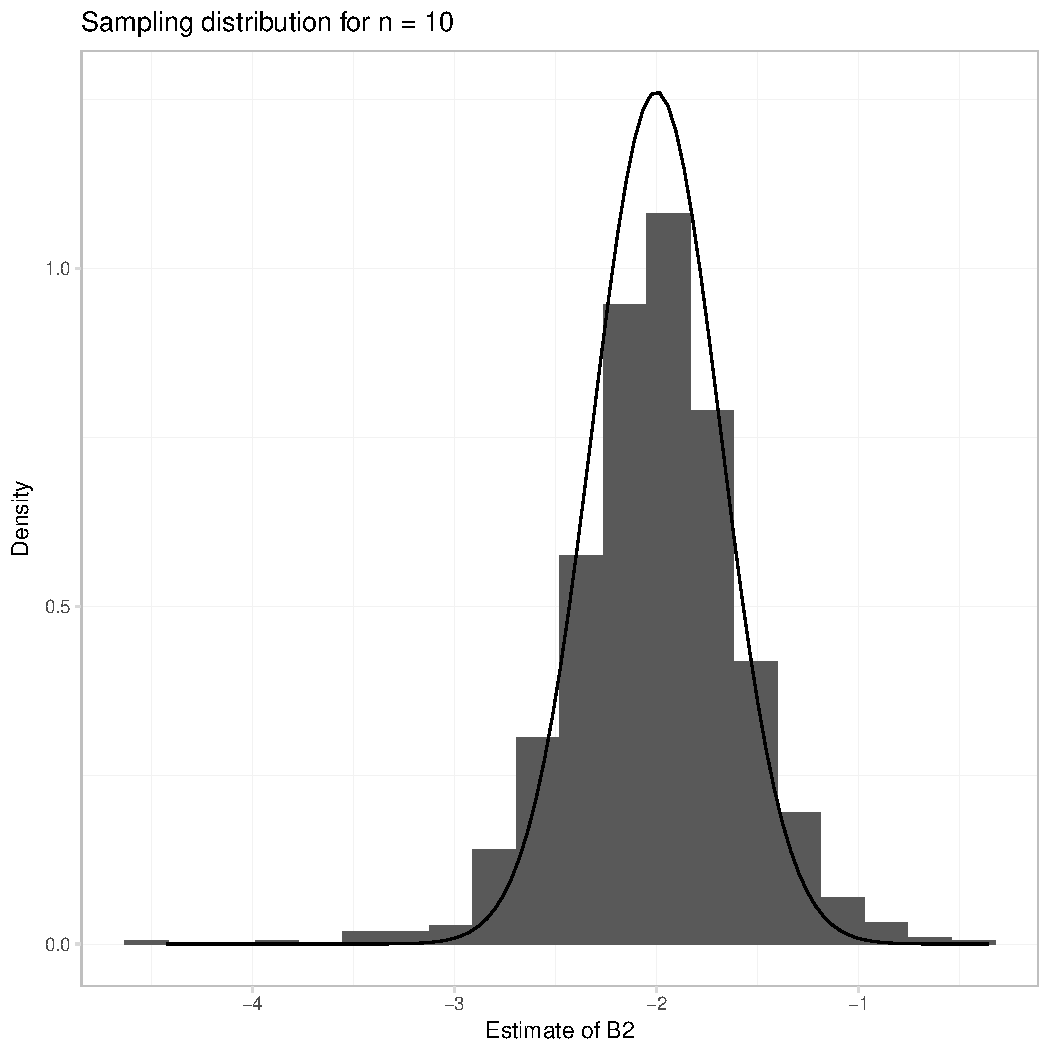
\includegraphics[width=\maxwidth]{figure/Q2_looping-1} 

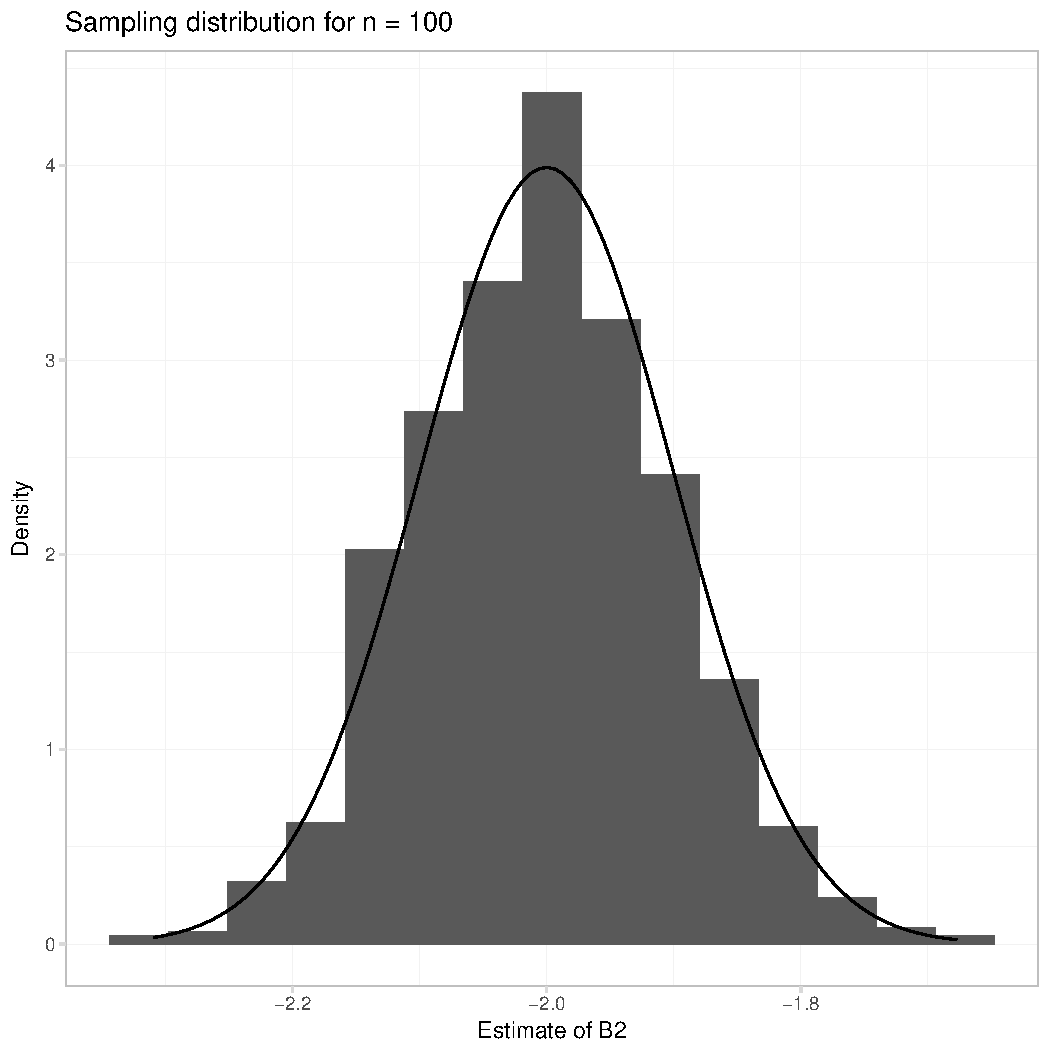
\includegraphics[width=\maxwidth]{figure/Q2_looping-2} 

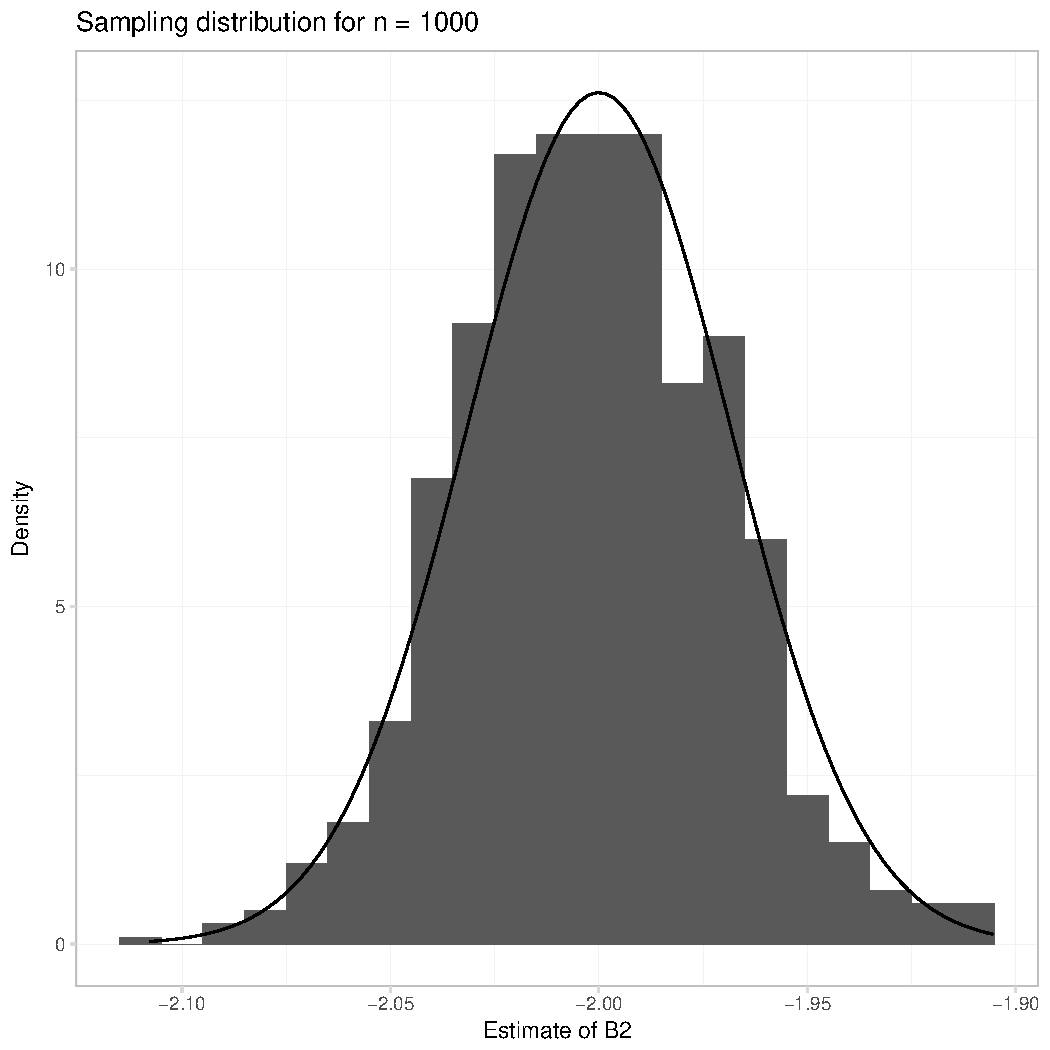
\includegraphics[width=\maxwidth]{figure/Q2_looping-3} 

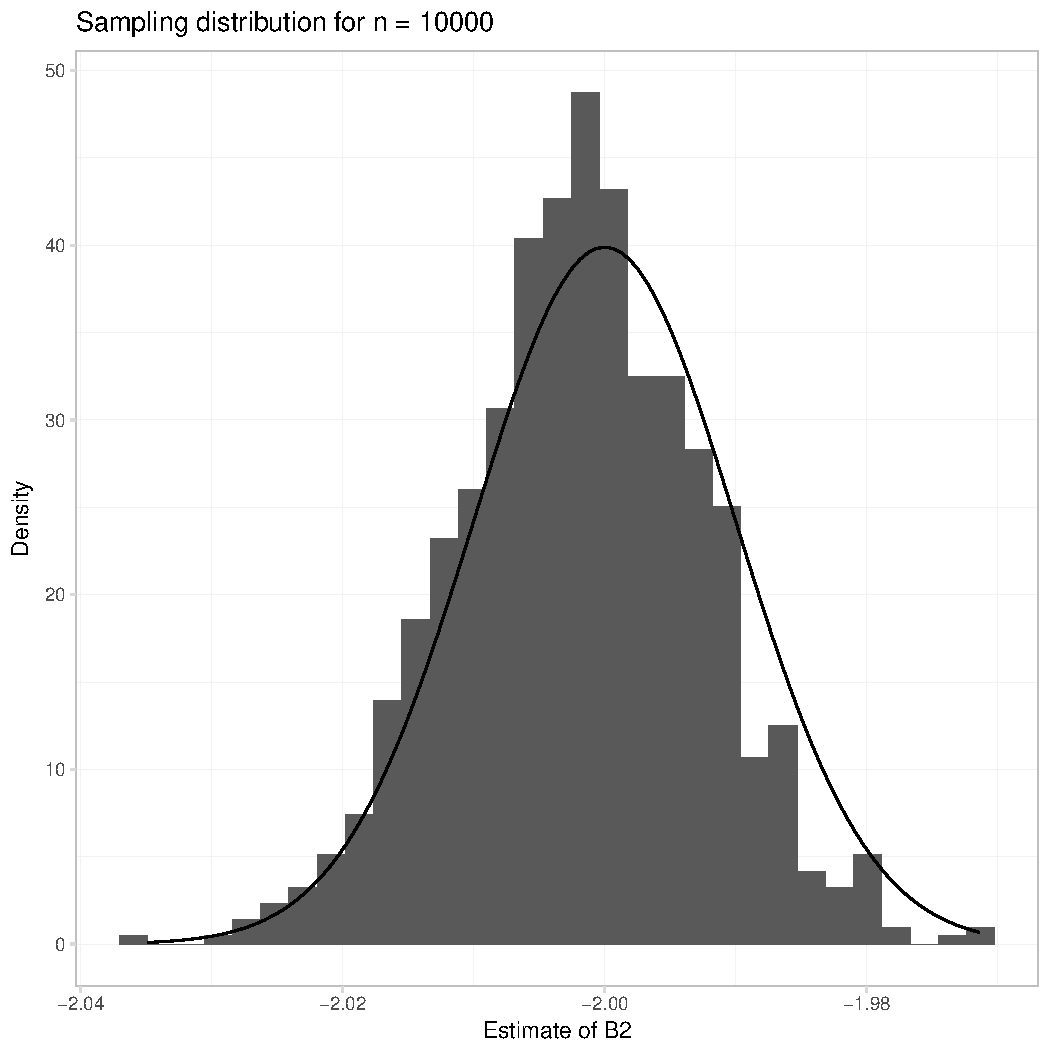
\includegraphics[width=\maxwidth]{figure/Q2_looping-4} 

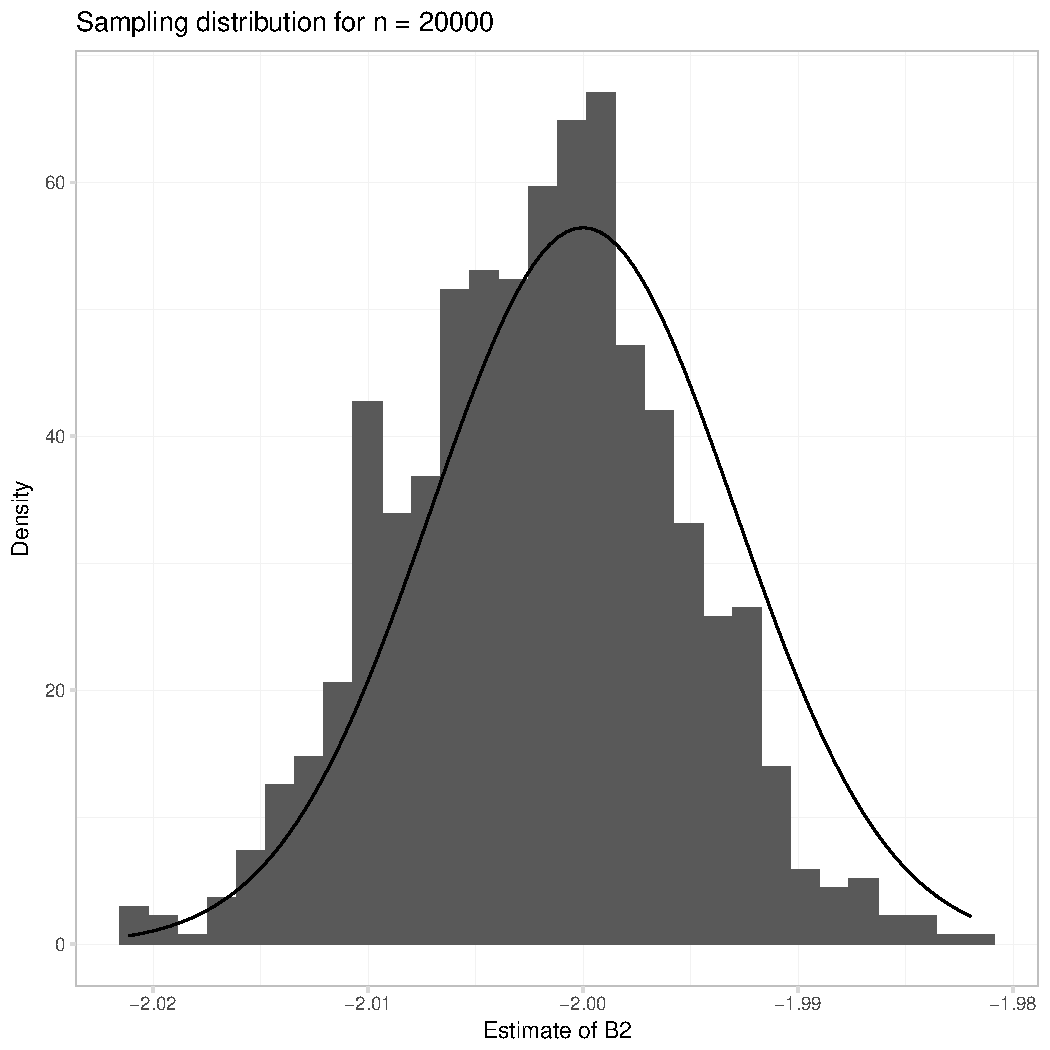
\includegraphics[width=\maxwidth]{figure/Q2_looping-5} 

\end{knitrout}


\newpage
\noindent \section*{Question 2 Part B}
\noindent For this part we change the ols function to use the appropriate y, and adjust the variance of the normal distribution to reflect the fact that $\eta$ has a different variance than $\epsilon$.  


\begin{knitrout}\footnotesize
\definecolor{shadecolor}{rgb}{0.969, 0.969, 0.969}\color{fgcolor}\begin{kframe}
\begin{alltt}
\hlcom{# Part B ---- }

\hlcom{# Just need to change up what we feed the ols function! }
\hlcom{# Also note that the asymptotic variance is also different: }
\hlcom{# v is going to be 1/12(8.66^2)=6.24963}
\hlcom{# z1/v2 is 5/6.24963 = 0.8}

\hlstd{one_iter} \hlkwb{<-} \hlkwa{function}\hlstd{(}\hlkwc{iter}\hlstd{,} \hlkwc{population}\hlstd{,} \hlkwc{size}\hlstd{) \{}
  \hlstd{sample_df} \hlkwb{<-} \hlkwd{sample_n}\hlstd{(}\hlkwc{tbl} \hlstd{= population, size)}

  \hlcom{# Calculate the OLS coefficient }
  \hlstd{coef_ols} \hlkwb{<-} \hlkwd{b_ols}\hlstd{(}
    \hlkwc{y} \hlstd{=} \hlkwd{to_matrix}\hlstd{(sample_df,} \hlstr{"y_b"}\hlstd{),}
    \hlkwc{X} \hlstd{=} \hlkwd{to_matrix}\hlstd{(sample_df,} \hlkwd{c}\hlstd{(}\hlstr{"i"}\hlstd{,} \hlstr{"x1"}\hlstd{,} \hlstr{"x2"}\hlstd{)))}

  \hlcom{# Create a return a dataframe }
  \hlstd{coef_df} \hlkwb{<-} \hlkwd{data.frame}\hlstd{(}
    \hlkwc{est}    \hlstd{=} \hlkwd{as.vector}\hlstd{(coef_ols),}
    \hlkwc{param}  \hlstd{=} \hlkwd{c}\hlstd{(}\hlstr{"int"}\hlstd{,} \hlstr{"b1"}\hlstd{,} \hlstr{"b2"}\hlstd{),}
    \hlkwc{iter}   \hlstd{= iter}
  \hlstd{)}
  \hlcom{# Return the data.frame}
  \hlkwd{print}\hlstd{(coef_ols)}
  \hlkwd{return}\hlstd{(coef_df)}
\hlstd{\}}


\hlcom{# repeating for all sample sizes: }
\hlstd{n_list}\hlkwb{<-}\hlkwd{c}\hlstd{(}\hlnum{10}\hlstd{,} \hlnum{100}\hlstd{,} \hlnum{1000}\hlstd{,} \hlnum{10000}\hlstd{,} \hlnum{20000}\hlstd{)}
\hlkwa{for} \hlstd{(n} \hlkwa{in} \hlstd{n_list) \{}
  \hlstd{sim_df} \hlkwb{<-} \hlkwd{parLapply}\hlstd{(}
    \hlkwc{cl} \hlstd{= cl,}
    \hlkwc{X} \hlstd{=} \hlnum{1}\hlopt{:}\hlnum{1000}\hlstd{,}
    \hlkwc{fun} \hlstd{= one_iter,}
    \hlkwc{population} \hlstd{= data_df,} \hlkwc{size}\hlstd{=n)} \hlopt \hlkwd{bind_rows}\hlstd{()} \hlopt \hlkwd{tbl_df}\hlstd{()}

  \hlcom{# Plot a separate histogram of the estimated B2’s for each sample size: }

  \hlstd{plot_data}\hlkwb{<-}\hlkwd{subset}\hlstd{(sim_df,  param} \hlopt{==} \hlstr{"b2"}\hlstd{)}
  \hlstd{plot}\hlkwb{<-}\hlkwd{ggplot}\hlstd{(plot_data,} \hlkwd{aes}\hlstd{(est))} \hlopt{+}
    \hlcom{# Add normal dist with appropriate variance:}
    \hlkwd{geom_histogram}\hlstd{(}\hlkwd{aes}\hlstd{(}\hlkwc{y} \hlstd{= ..density..),} \hlkwc{binwidth} \hlstd{=} \hlnum{1}\hlopt{/}\hlstd{(n}\hlopt{^}\hlstd{(}\hlnum{2}\hlopt{/}\hlnum{3}\hlstd{)))} \hlopt{+}
    \hlkwd{stat_function}\hlstd{(}\hlkwc{fun} \hlstd{= dnorm,} \hlkwc{args} \hlstd{=} \hlkwd{list}\hlstd{(}\hlkwc{mean} \hlstd{=} \hlopt{-}\hlnum{2}\hlstd{,} \hlkwc{sd} \hlstd{=} \hlnum{.8}\hlopt{/}\hlkwd{sqrt}\hlstd{(n)))} \hlopt{+}
    \hlkwd{xlab}\hlstd{(}\hlstr{"Estimate of B2"}\hlstd{)} \hlopt{+}
    \hlkwd{ylab}\hlstd{(}\hlstr{"Density"}\hlstd{)} \hlopt{+}
    \hlkwd{ggtitle}\hlstd{(}\hlkwd{paste}\hlstd{(}\hlstr{"Sampling distribution for n ="}\hlstd{,} \hlkwd{as.character}\hlstd{(n)))}\hlopt{+}
    \hlstd{theme}

  \hlstd{plot}
  \hlkwd{print}\hlstd{(plot)}
\hlstd{\}}
\end{alltt}
\end{kframe}
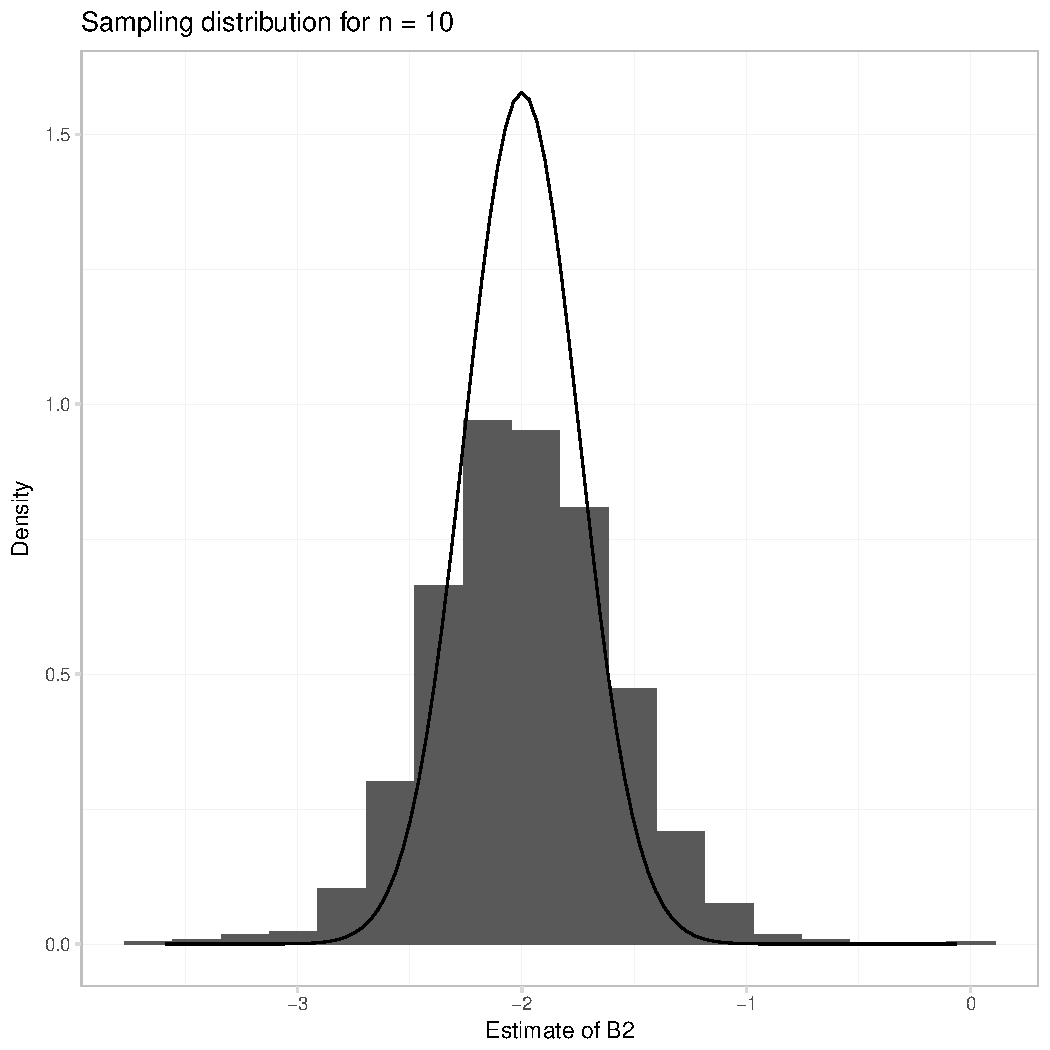
\includegraphics[width=\maxwidth]{figure/Part_B-1} 

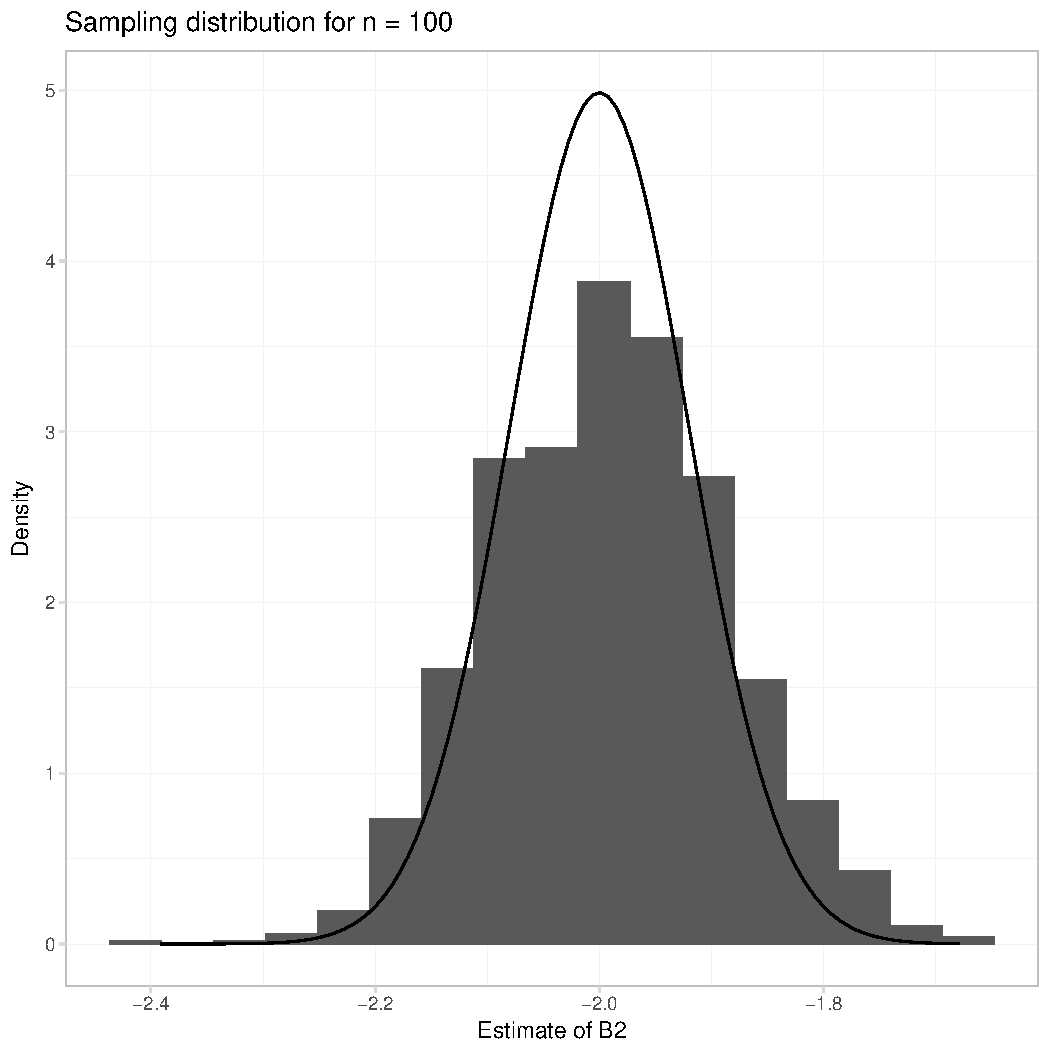
\includegraphics[width=\maxwidth]{figure/Part_B-2} 

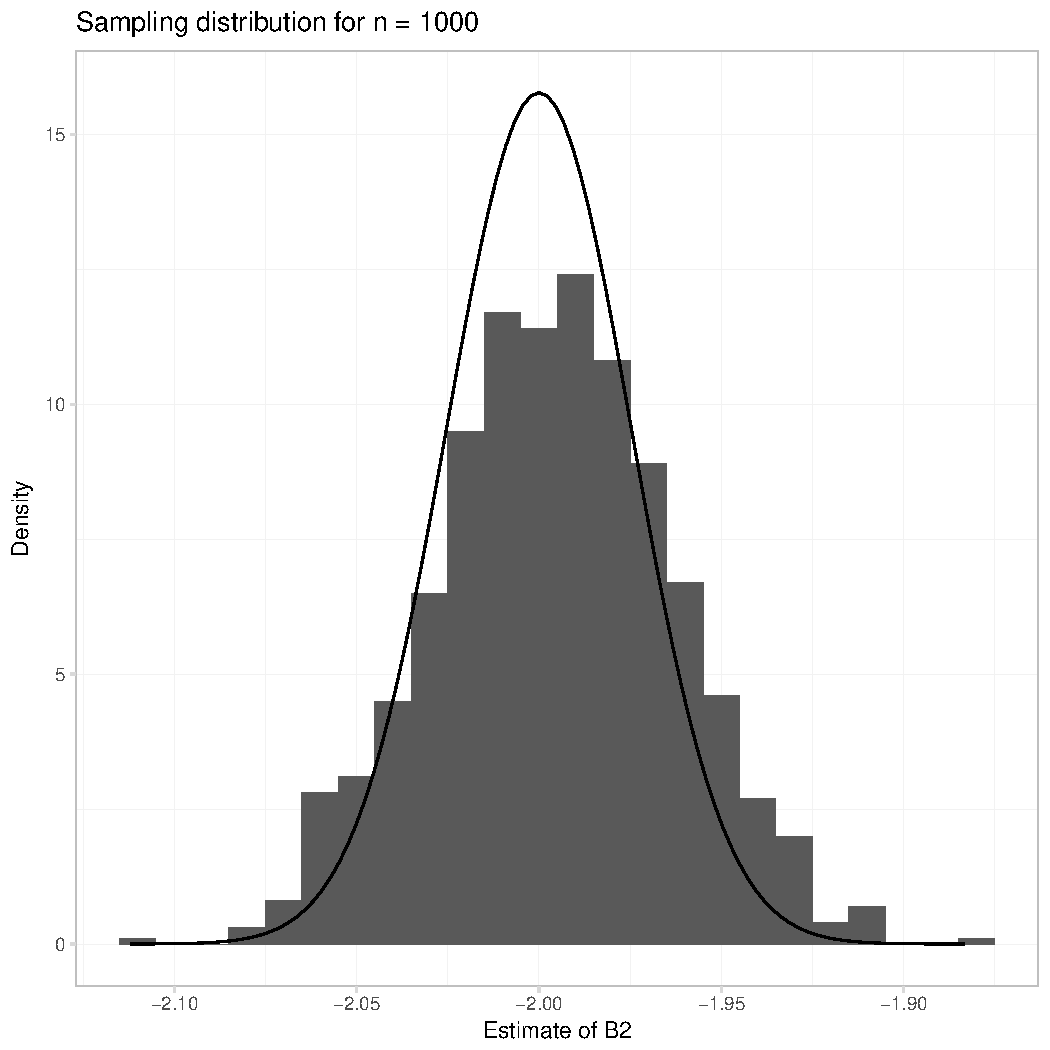
\includegraphics[width=\maxwidth]{figure/Part_B-3} 

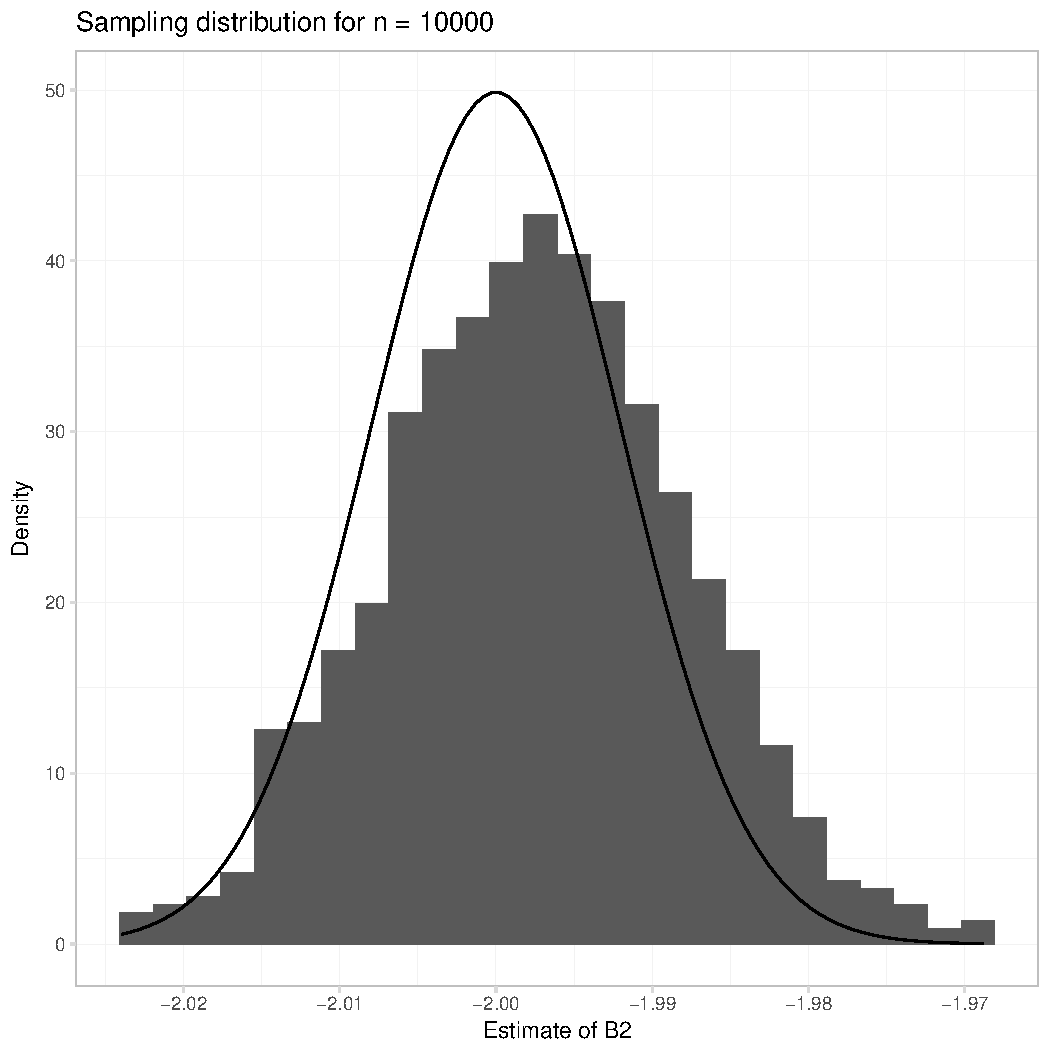
\includegraphics[width=\maxwidth]{figure/Part_B-4} 

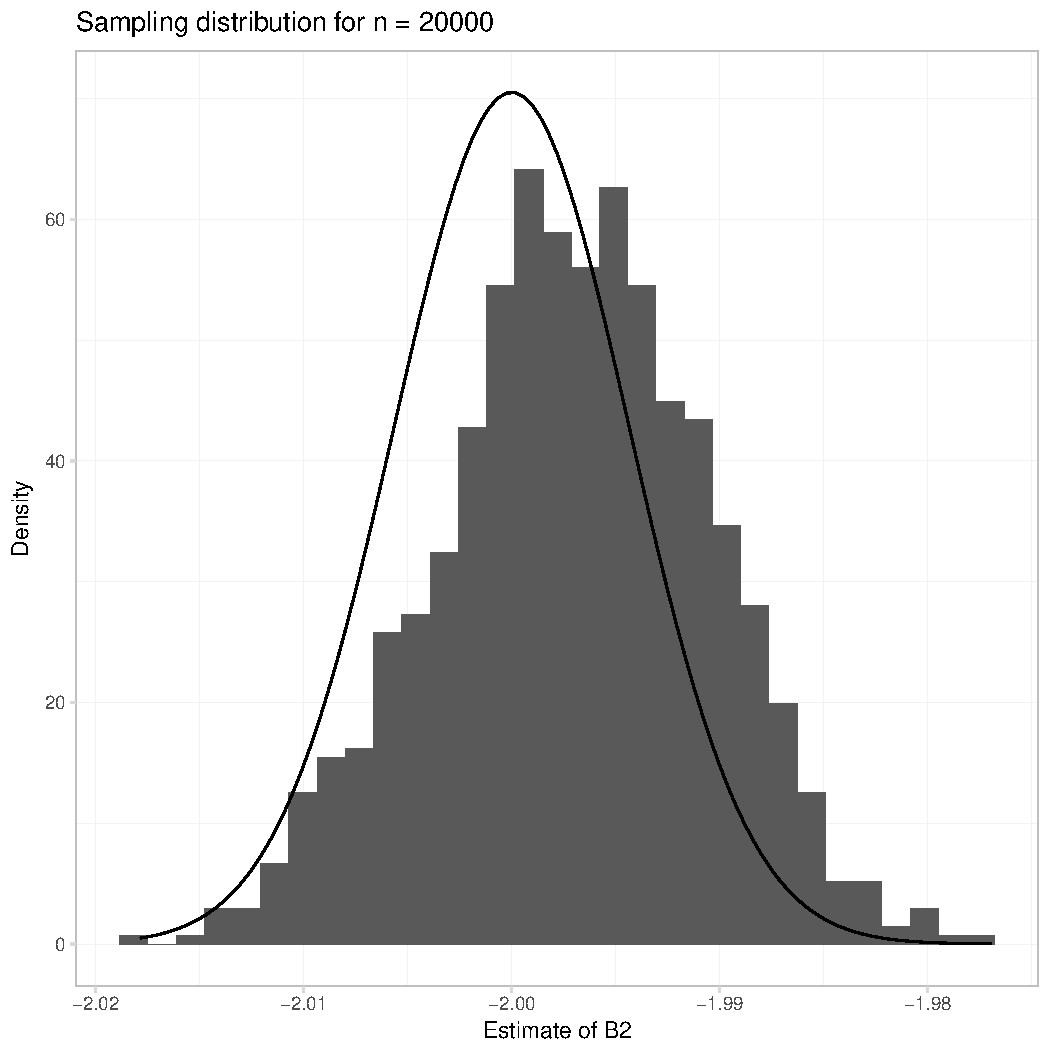
\includegraphics[width=\maxwidth]{figure/Part_B-5} 

\end{knitrout}

We can see that as sample size increases, the distribution of $\beta_{2}$ approaches the overlayed normal distribution. This is true even in Part B, where the errors are not normall distributed. For a very large sample, however, the distribution doesn't line up exactly with the histogram. This is because the 'population' was itself a random sample, and thus the \textit{true} value for the coefficient in the population from which we sample is not -2. 

\end{document}


















